\documentclass[a4paper,11pt]{article}

\usepackage{bsymb}
\usepackage[T1]{fontenc} % utf8
\usepackage[utf8]{inputenc} % utf8
\usepackage[german]{babel} % deutsche silbentrennung

\title{__OUTFILE_TITLE__}
\author{Jochen Peters}

\usepackage[
 pdftitle={__OUTFILE_TITLE__},
 pdfauthor={Jochen Peters}
]{hyperref}

\date{\today}

\usepackage{cite}
\usepackage{amsmath}
\usepackage{array}
\usepackage{url}

\usepackage[pdftex]{graphicx}
\usepackage{color,xcolor,colortbl}
\usepackage{picture}

% start - scale image if needed
\makeatletter
\def\ScaleIfNeeded{%
  \ifdim\Gin@nat@width>\linewidth
    \linewidth
  \else
    \Gin@nat@width
  \fi
}
\makeatother
\setkeys{Gin}{width=\ScaleIfNeeded}
% end - scale image if needed

% code einbinden / hightlight
\usepackage{minted}

\setminted{fontsize=\small,baselinestretch=1,linenos,breaklines}

% macht aus \begin{minted}{cpp} -> \begin{cppcode}  bzw \end
\newminted{cpp}{
% frame=lines,
% framesep=2mm,
 baselinestretch=1.2,
 fontsize=\footnotesize,
 linenos}
\newminted{bash}{
% frame=lines,
% framesep=2mm,
 baselinestretch=1.2,
 fontsize=\footnotesize,
 linenos}

\usepackage[cm]{fullpage}  % mit 1,5cm rand

\usepackage{longtable}
\usepackage{booktabs} % enhance the quality of tables

\parskip3pt{}
\parindent0mm{} % einrueckung absatzanfang
\textheight24cm{}
\textwidth16cm{}
\oddsidemargin0mm{}
\topmargin-10mm{}

\providecommand{\tightlist}{%
   \setlength{\itemsep}{0pt}\setlength{\parskip}{0pt}}

\begin{document}

\maketitle
\tableofcontents

\hypertarget{motivation}{%
\section{Motivation}\label{motivation}}

\begin{frame}{To Get or To Become a Part of the Hadoop Tart}
\protect\hypertarget{to-get-or-to-become-a-part-of-the-hadoop-tart}{}

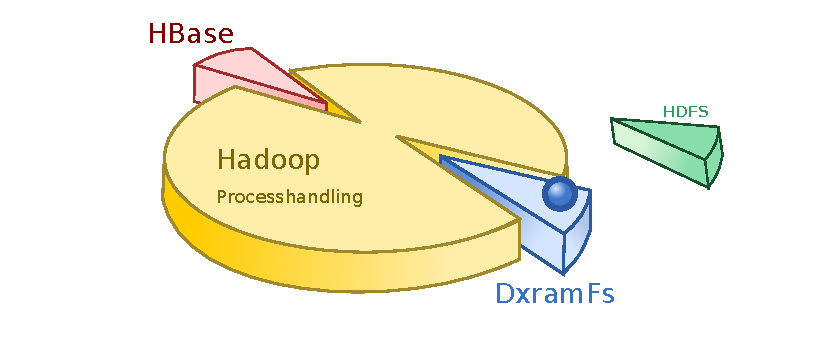
\includegraphics{fig/introtart.pdf}

\end{frame}

\begin{frame}{DXRAM usage}
\protect\hypertarget{dxram-usage}{}

\begin{itemize}
\tightlist
\item
  join to other popular Distrubuted Systems
\item
  DXRAM as alternative storage system
\item
  enlarge DXRAM popularity
\end{itemize}

\end{frame}

\begin{frame}{DXRAM usage}
\protect\hypertarget{dxram-usage-1}{}

Idea: become a part of a popular project

\begin{itemize}
\tightlist
\item
  Hadoop
\item
  HBase
\end{itemize}

Big Vision: remove HDFS access in HBase by DXRAM

\end{frame}

\begin{frame}{Excursion Hadoop}
\protect\hypertarget{excursion-hadoop}{}

\textbf{Hadoop}

\end{frame}

\begin{frame}{Excursion Hadoop}
\protect\hypertarget{excursion-hadoop-1}{}

\begin{itemize}
\tightlist
\item
  starts with HDFS: split big files into big blocks
\item
  a block maybe replicated
\item
  Namenode: stores Blocklocations and infrastructure info
\item
  MapReduce: split \emph{Job} into \emph{Tasks} on blocks
\item
  becomes more and more a process handling ``ecosystem'' (YARN)
\end{itemize}

Run Task where data block is stored.

\end{frame}

\begin{frame}{Excursion Hadoop - Sketch}
\protect\hypertarget{excursion-hadoop---sketch}{}

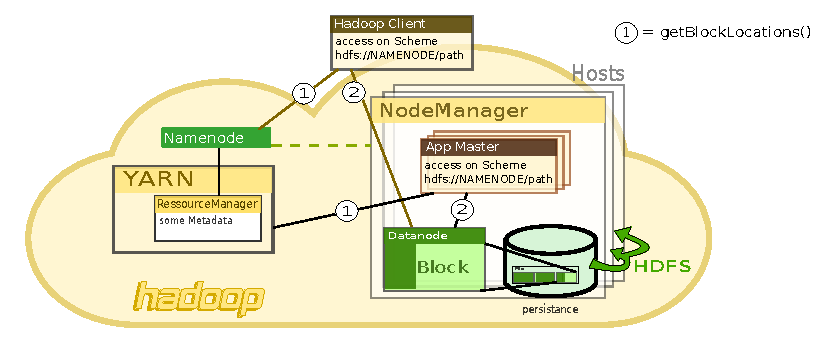
\includegraphics{fig/hadoop.pdf}

\end{frame}

\begin{frame}{Excursion HBase}
\protect\hypertarget{excursion-hbase}{}

\textbf{Hbase}

\end{frame}

\begin{frame}{Excursion HBase}
\protect\hypertarget{excursion-hbase-1}{}

\begin{itemize}
\tightlist
\item
  noSQL with BASE and not ACID (SQL)
\item
  store in RAM, but a WAL for persistance
\item
  HDFS for WAL and flushes
\item
  hard to balance (optimal for read OR write)
\item
  each node has some RegionServer (handle key region for each column
  family)
\end{itemize}

\end{frame}

\begin{frame}{Exkurs HBase - Sketch}
\protect\hypertarget{exkurs-hbase---sketch}{}

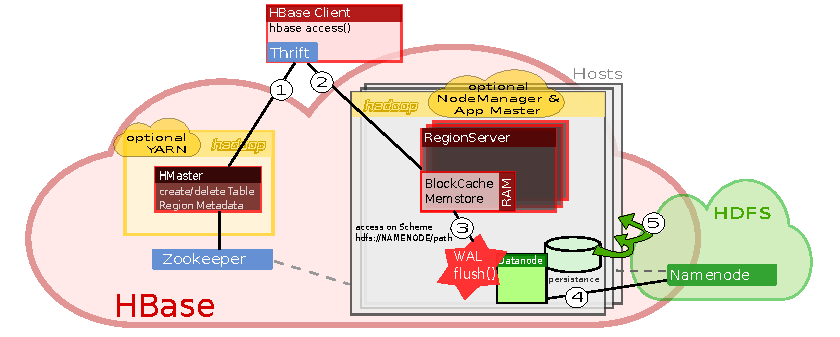
\includegraphics{fig/hbase.pdf}

\end{frame}

\begin{frame}{HBase and DXRAM}
\protect\hypertarget{hbase-and-dxram}{}

\textbf{HBase and DXRAM ?}

\end{frame}

\begin{frame}{HBase and DXRAM}
\protect\hypertarget{hbase-and-dxram-1}{}

\begin{itemize}
\tightlist
\item
  HBase uses MemStore \& BlockCache (RAM)
\item
  WAL: does an ACK after writing change to HDFS
\item
  big focus on persistence and data compaction
\item
  NoSQL: waiting for hard disk on writing? any benefit to normal SQL?
\end{itemize}

Why not using DXRAM as distributed RAM instead of harddisk, WAL and
compaction processes?

\end{frame}

\hypertarget{other-hadoop-friendly-ram-stores}{%
\section{Other Hadoop friendly RAM
stores}\label{other-hadoop-friendly-ram-stores}}

\begin{frame}{Other Hadoop friendly RAM stores}
\protect\hypertarget{other-hadoop-friendly-ram-stores-1}{}

Distributed Memory and Hadoop + HBase:

\textbf{How does other projects handle this?}

\end{frame}

\begin{frame}[fragile]{Other Hadoop friendly RAM stores}
\protect\hypertarget{other-hadoop-friendly-ram-stores-2}{}

Ignite:

\begin{itemize}
\tightlist
\item
  distributed key-value storage
\item
  has an optional SQL engine
\item
  sees itself as a competition to HBase
\item
  optional WAL for recovery: local FS
\item
  has a Hadoop FS Connector \texttt{igfs://}
\item
  optional \texttt{igfs} persistence: \texttt{hdfs://}
\end{itemize}

\end{frame}

\begin{frame}{Ignite - Grafik}
\protect\hypertarget{ignite---grafik}{}

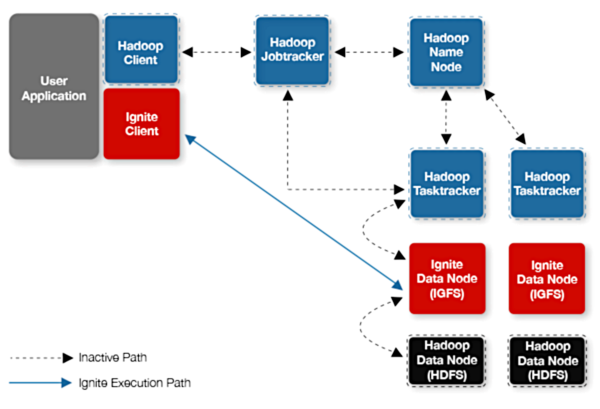
\includegraphics{fig/ignite.pdf}

\end{frame}

\begin{frame}[fragile]{Other Hadoop friendly RAM stores}
\protect\hypertarget{other-hadoop-friendly-ram-stores-3}{}

Alluxio:

\begin{itemize}
\tightlist
\item
  Code looks like a Hadoop \glqq{}Branch''
\item
  instead of Hadoop Scheme: mount into \texttt{alluxio://tree}
\item
  can work as a distributed FS cache
\item
  persistence is an optional FS feature

  \begin{itemize}
  \tightlist
  \item
    Under Storage: local FS
  \end{itemize}
\item
  has a Hadoop FS Connector
\item
  FS Connector usable in HBase, too
\end{itemize}

\end{frame}

\begin{frame}{Alluxio - Grafik}
\protect\hypertarget{alluxio---grafik}{}

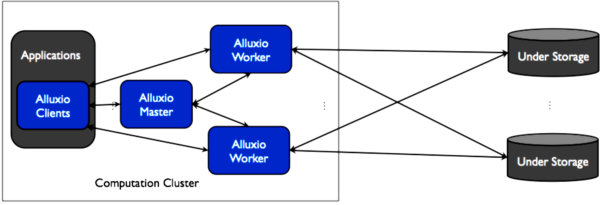
\includegraphics{fig/alluxio.pdf}

\end{frame}

\hypertarget{approaches}{%
\section{Approaches}\label{approaches}}

\begin{frame}{Approaches}
\protect\hypertarget{approaches-1}{}

\textbf{Solutions to use DXRAM in Hadoop and HBase}

\end{frame}

\begin{frame}{I: DXRAM.Base}
\protect\hypertarget{i-dxram.base}{}

HBase Replacement based on the Thrift IDL for HBase Clients

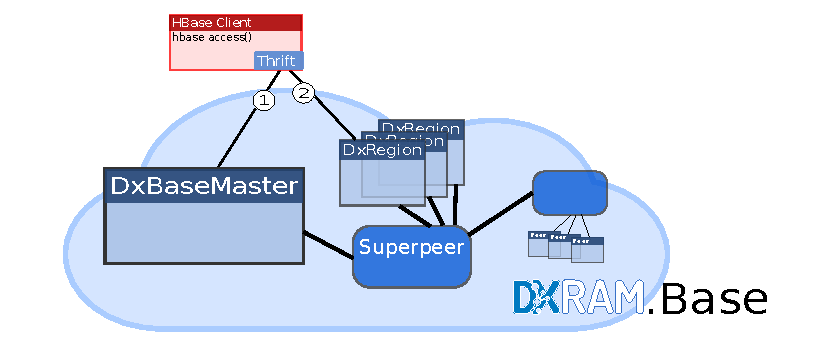
\includegraphics{fig/replacement.pdf}

\end{frame}

\begin{frame}{I: DXRAM.Base}
\protect\hypertarget{i-dxram.base-1}{}

\textbf{Pro}

\begin{itemize}
\tightlist
\item
  maximal freedom to implement this
\item
  maybe the most efficient way
\item
  Hadoop independent
\end{itemize}

\end{frame}

\begin{frame}{I: DXRAM.Base}
\protect\hypertarget{i-dxram.base-2}{}

\textbf{Contra}

\begin{itemize}
\tightlist
\item
  unclear how HBase and the Hadoop community react to it
\item
  the community may not want renounce Hadoop
\item
  other Hadoop projects have low benefit from it
\end{itemize}

\end{frame}

\begin{frame}{II: RegionServer Mod}
\protect\hypertarget{ii-regionserver-mod}{}

RegionServer RAM access modified with DXRAM stuff.

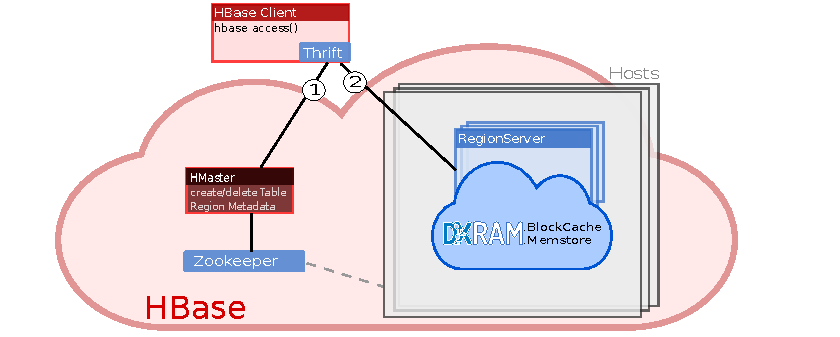
\includegraphics{fig/regionserverMod.pdf}

\end{frame}

\begin{frame}{II: RegionServer Mod}
\protect\hypertarget{ii-regionserver-mod-1}{}

\textbf{Pro}

\begin{itemize}
\tightlist
\item
  optimized for HBase
\item
  Hadoop independent
\item
  maybe better compatibility than a complete HBase replacement
\end{itemize}

\end{frame}

\begin{frame}{II: RegionServer Mod}
\protect\hypertarget{ii-regionserver-mod-2}{}

\textbf{Contra}

\begin{itemize}
\tightlist
\item
  deep know-how about code and HBase procedures necessary
\item
  HBase Updates got in trouble
\item
  other Hadoop projects have low benefit from it
\end{itemize}

\end{frame}

\begin{frame}[fragile]{III: Mounting DXRAM}
\protect\hypertarget{iii-mounting-dxram}{}

Mount DXRAM as RAM-Drive with \texttt{libfuse}

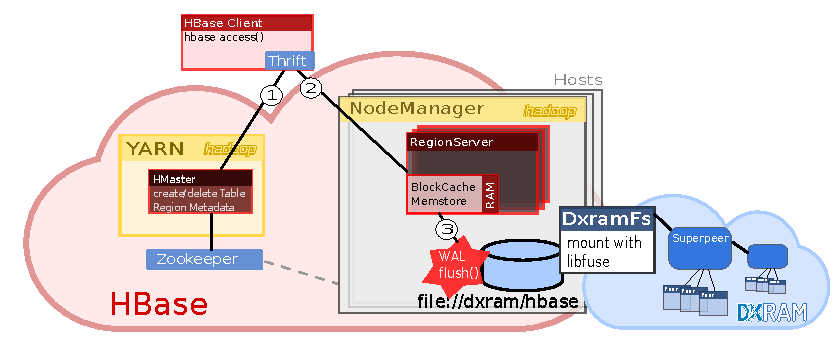
\includegraphics{fig/mountable.pdf}

\end{frame}

\begin{frame}{III: Mounting DXRAM}
\protect\hypertarget{iii-mounting-dxram-1}{}

\textbf{Pro}

\begin{itemize}
\tightlist
\item
  No HBase or Hadoop code have to been changed or added
\item
  effect on all projects, using local FS for persistance and recovery
\end{itemize}

\end{frame}

\begin{frame}[fragile]{III: Mounting DXRAM}
\protect\hypertarget{iii-mounting-dxram-2}{}

\textbf{Contra}

\begin{itemize}
\tightlist
\item
  Hadoop loses information about block locations. Host based Task
  splitting inpossible
\item
  Performance leaks with \texttt{libfuse}
\item
  a bit complicated: build a NFS like filesystem with distributed block
  location
\end{itemize}

\end{frame}

\begin{frame}{IV: DXRAM FS Connector}
\protect\hypertarget{iv-dxram-fs-connector}{}

Like Ignite and Alluxio: build a DXRAM FS Connector.

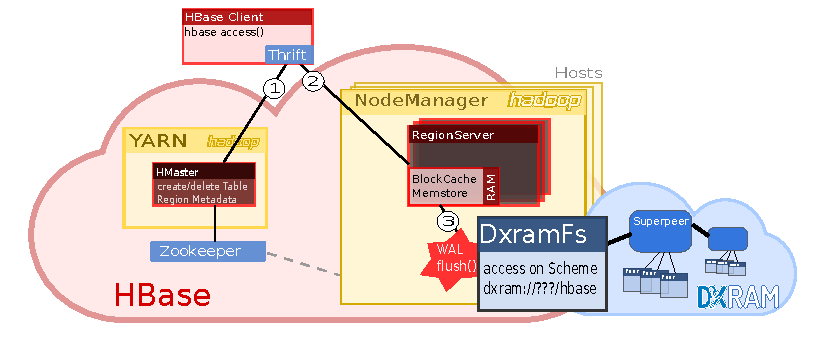
\includegraphics{fig/dxramconnector.pdf}

\end{frame}

\begin{frame}{IV: DXRAM FS Connector}
\protect\hypertarget{iv-dxram-fs-connector-1}{}

\textbf{Pro}

\begin{itemize}
\tightlist
\item
  Modular addable to HBase and Hadoop
\item
  benefit for all Hadoop projects without modifications
\item
  Hadoops Host based Task splitting is possible
\end{itemize}

\end{frame}

\begin{frame}{IV: DXRAM FS Connector}
\protect\hypertarget{iv-dxram-fs-connector-2}{}

\textbf{Contra}

Big Milestones:

\begin{itemize}
\tightlist
\item
  build a FS based on DXRAM
\item
  make FS similar to the block based HDFS
\item
  transport data from DXRAM Application to an alien like Hadoop
\end{itemize}

\end{frame}

\begin{frame}{Election}
\protect\hypertarget{election}{}

The choice fell on the DXRAM FS Connector, because it offers the widest
range of uses.

\end{frame}

\hypertarget{implementation}{%
\section{Implementation}\label{implementation}}

\begin{frame}{Implementation}
\protect\hypertarget{implementation-1}{}

\begin{itemize}
\tightlist
\item
  DxramFs App: Chunks are similar to blocks
\item
  DXNET: RPC and data transport
\item
  DxramFs Connector: Hadoop uses DXNET
\item
  DXRAM not part of HBase or Hadoop
\end{itemize}

\end{frame}

\begin{frame}{Implementation - Sketch}
\protect\hypertarget{implementation---sketch}{}

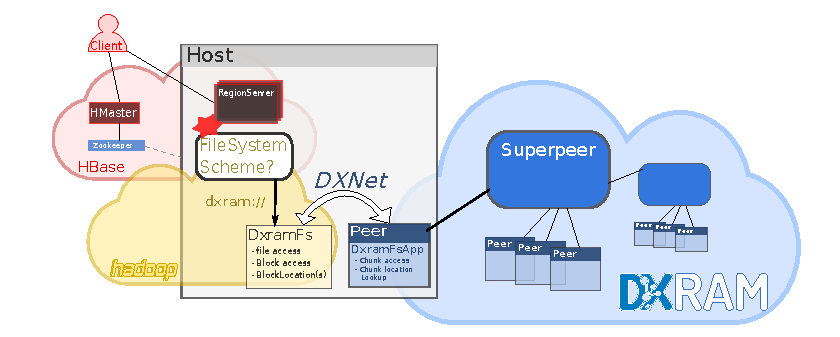
\includegraphics{fig/done.pdf}

\end{frame}

\begin{frame}{Implementation :-(}
\protect\hypertarget{implementation--}{}

Project failed primarily because of debugging effort in serializing pure
attribute classes.

\end{frame}

\begin{frame}{Implementation: Fail 1}
\protect\hypertarget{implementation-fail-1}{}

\begin{figure}
\centering
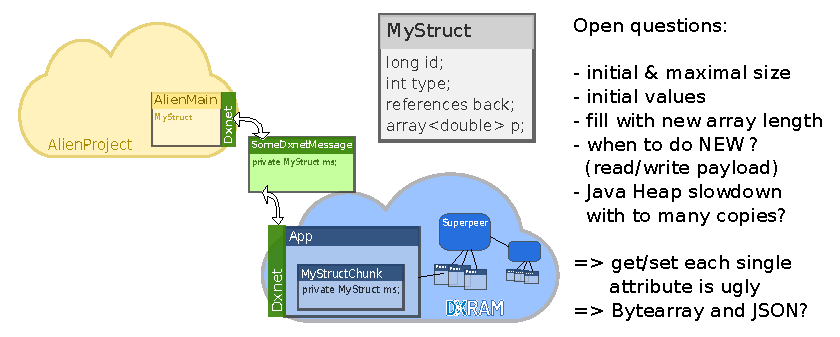
\includegraphics{fig/structUgly.pdf}
\caption{wihout wrapper or preprocessing}
\end{figure}

\end{frame}

\begin{frame}{Implementation: Fail 1}
\protect\hypertarget{implementation-fail-1-1}{}

\begin{itemize}
\tightlist
\item
  inital values, different size with new data
\item
  a IDL like Apache Thrift would be nice
\end{itemize}

\end{frame}

\begin{frame}{DXRAM feature request}
\protect\hypertarget{dxram-feature-request}{}

\begin{figure}
\centering
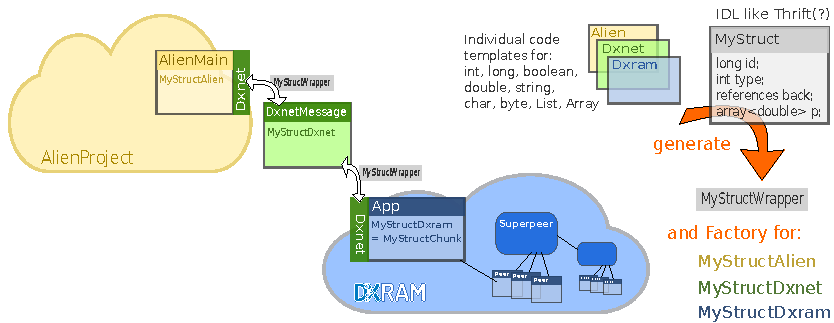
\includegraphics{fig/structAPI.pdf}
\caption{with preprocessing}
\end{figure}

\end{frame}

\begin{frame}{Implementation: Fail 2}
\protect\hypertarget{implementation-fail-2}{}

The next mistake: slicing up the multipeer use-case

\end{frame}

\begin{frame}{Implementation: Fail 2}
\protect\hypertarget{implementation-fail-2-1}{}

Single peer on localhost is a bad testing scene:

\begin{itemize}
\tightlist
\item
  Questions about an Alien Node to DXRAM Node mapping answered to late
\item
  Hadoop Task splitting still not tested
\item
  errors caused by wrong stored Chunks occours next to project end
\end{itemize}

Instead of building a local FS connector as a first test, I should have
better converted the Hadoop FTP connector to Multipeer szenario.

\end{frame}

\begin{frame}{Implementation: DXNET Transport}
\protect\hypertarget{implementation-dxnet-transport}{}

Is it optimal? Hadoop transfer jobs to local data, thus DXNET doing
network traffic just on localhost.

\end{frame}

\begin{frame}{Implementation: Now}
\protect\hypertarget{implementation-now}{}

\textbf{Finished:} FS structure, operations on directories

\end{frame}

\begin{frame}[fragile]{Implementation: Now}
\protect\hypertarget{implementation-now-1}{}

\textbf{still open}

\begin{itemize}
\tightlist
\item
  bugs on storing and sharing chunks between peers
\item
  starting with: \texttt{create}, \texttt{open}, \texttt{flush},
  \texttt{In-} and \texttt{OutStream}
\item
  small bugs in copy and rename (see website)
\item
  big FS contents, really big file handling
\item
  handling multiple DXNET RPCalls
\end{itemize}

\end{frame}

\begin{frame}{Implementation: Now}
\protect\hypertarget{implementation-now-2}{}

\textbf{far away}

\begin{itemize}
\tightlist
\item
  ATOMar FS access, Hadoop unit tests
\item
  test with MapReduce and HBase code examples
\item
  performance tests
\end{itemize}

\end{frame}

\hypertarget{conclusion}{%
\section{Conclusion}\label{conclusion}}

\begin{frame}{Conclusion}
\protect\hypertarget{conclusion-1}{}

\begin{itemize}
\tightlist
\item
  Ignite \& Alluxio: Doing a YARN replacement
\item
  Hadoop ecosystem is too close to HDFS block handling
\item
  Is it easier to build a distributed noSQL Database than a distributed
  FS with an key-value store?!
\end{itemize}

\end{frame}

\begin{frame}{Conclusion}
\protect\hypertarget{conclusion-2}{}

BUT: \textbf{nobody} advertises to \textbf{replace} HBase or Hadoop, but
to be able to \textbf{cooperate} with them.

\end{frame}

\begin{frame}{Questions}
\protect\hypertarget{questions}{}

Questions?

\end{frame}

\begin{frame}{Questions}
\protect\hypertarget{questions-1}{}

Thank you for your attention.

\end{frame}

\begin{frame}{References}
\protect\hypertarget{references}{}

You got everything on
\href{https://no-go.github.io/HadoopDxramFS}{no-go.github.io/HadoopDxramFS}.

\end{frame}


\end{document}
